\section{模型评价、稳健性分析与推广}

\subsection{模型优点}

\begin{enumerate}
    \item \textbf{公共口径统一、逐问可继承}。全文共用同一套 DEM 采样、能耗公式、两阶段充电与作业时间引擎，问题一至四的能耗/时间/架次指标口径一致，问题间的数据继承关系明确，结果可直接横向比较。
    \item \textbf{多方法交叉验证}。问题一用线性加权、Chebyshev 妥协、NSGA-II 三种方法收敛于同一方案（$N=18$）；问题二、三、四分别以"构造式 + 全局优化"或"精确枚举 + 局部搜索"两套方法互相校验，显著增强了结果的可靠性。
    \item \textbf{精确与启发式分层}。问题一的集合划分 MILP 与问题四的完全枚举在给定规模内取得全局最优；当规模增大时以 NSGA-II 或模拟退火局部搜索保持可扩展性，兼顾了最优性与可解性。
    \item \textbf{物理机理严谨}。能耗由航程包络反推、爬升能耗由重力势能推导、通信由自由空间损耗与 DEM 遮挡判定、充电用两阶段非线性模型，均与题设及公开文献\cite{ref_zhang,ref_itu,ref_ti}一致。
    \item \textbf{结果可复现、自检完整}。每个求解脚本均内置覆盖校验（80/80 箱、质量/体积守恒、无超容批次）与跨引擎自检（多站能耗严格小于两次单站往返之和），保证结果可追溯。
\end{enumerate}

\subsection{算法复杂度与可扩展性分析}

表~\ref{tab:complexity} 汇总全文各问所采用算法的复杂度与适用规模。问题一的候选批次 DFS 枚举在 15 区 $\times$ 3 机型下仅产生 19525 个候选，集合划分 MILP 可直接精确求解；问题二的贪心合并为多项式时间、NSGA-II 的每代解码与离散事件仿真主导计算（种群 80、代数 80，实测约 64\,s）；问题三的中继候选网格枚举规模为 3420 个候选点，集合覆盖贪心分配为线性级；问题四的完全枚举规模随块数与 $K$ 呈第二类 Stirling 数（Bell 数）增长，$S(13,2)=4095$、$S(13,3)=261625$ 尚可枚举，但块数再增即不可行，此时以 $O(\text{iter}\cdot n)$ 的模拟退火局部搜索保持可解性。

\begin{table}[htbp]
\centering
\caption{全文各问算法复杂度与可扩展性}
\label{tab:complexity}
\small
\begin{tabular}{llll}
\toprule
\textbf{问题} & \textbf{算法} & \textbf{复杂度 / 规模} & \textbf{可扩展性} \\
\midrule
问题一 & DFS 候选枚举 + 集合划分 MILP & $|\mathcal{J}|=19525$，MILP 精确 & 精确，规模受限 \\
问题一 & NSGA-II + Minkowski 合并 & 各服务区局部前沿（$<200$） & 好 \\
问题二 & 贪心多站合并 & $O(n^2)$ 合并扫描，多项式 & 好，非全局最优 \\
问题二 & NSGA-II 全局优化 & $O(\text{pop}\cdot\text{gen}\cdot\text{解码}\cdot\text{仿真})$ & 好 \\
问题三 & 中继候选网格 + 集合覆盖 & 3420 候选点，贪心线性 & 好 \\
问题四 & 完全枚举 & $S(13,2)=4095$、$S(13,3)=261625$ & Bell 数增长，受限 \\
问题四 & 模拟退火局部搜索 & $O(\text{iter}\cdot n)$，300 轮 & 好 \\
\bottomrule
\end{tabular}
\end{table}

这一"精确与启发式分层"的设计使全文在给定规模内保证最优性（问题一 MILP、问题四枚举），在规模增大时保持可解性（NSGA-II、模拟退火），兼顾了最优性与可扩展性。

\subsection{模型缺点与改进方向}

\begin{enumerate}
    \item \textbf{NSGA-II 的架次与能耗代价偏高}。问题二主方案（NSGA-II）虽实现 0 硬约束违约，但为规避机身排队付出了更高架次（29 vs 16）与能耗（82.777 vs 58.179\,kWh）的代价；对比的贪心构造（16 架次）则存在 5 个硬时限违约。改进方向：在进化搜索中加入局部重排修复算子，或在贪心合并判据中显式加入硬时限松弛约束，以在架次与可行性之间取得更优折中。
    \item \textbf{完全枚举的均衡性与可扩展性受限}。问题四主方案（完全枚举）虽保证全局最优（缺口 1），但 K=3 组间均衡系数 0.3350 较差、且枚举规模随块数呈 Bell 数增长不可扩展；对比的局部搜索缺口 3/4 更大但 K=3 均衡性更好（0.0299）。改进方向：以精确解为初值做均衡性精修，或引入禁忌/变邻域搜索在更大规模下逼近最优并兼顾均衡。
    \item \textbf{中继悬停位置离散化}。中继位置在候选网格上搜索而非连续优化，可能遗漏连续最优悬停点。改进方向：在离散粗搜后用连续局部优化（如梯度法）精修悬停位置与高度。
    \item \textbf{通信遮挡判定偏保守}。相位内任一采样点被遮挡即判定全程需中继，会高估中继需求。改进方向：按子相位区间精细追踪遮挡时段，减少不必要的中继派遣。
    \item \textbf{电池资源池不含位置信息}。共享电池被建模为不带位置字段的全局时间戳资源，换电事实上被限制在 O01。改进方向：为电池引入位置状态，支持服务区就地换电，更贴近实际救援场景。
\end{enumerate}

\subsection{稳健性与交叉验证小结}

图~\ref{fig:compare_overview} 汇总了全文四问的模型方法对比：问题一三种方法收敛于同一方案；问题二刻画"少架次节能 vs 严格可行"；问题三量化通信保障的架次代价；问题四展示"精确最优 vs 可扩展近似"。该图直观呈现了各问方法对的取值差异与权衡方向。

\begin{figure}[htbp]
\centering
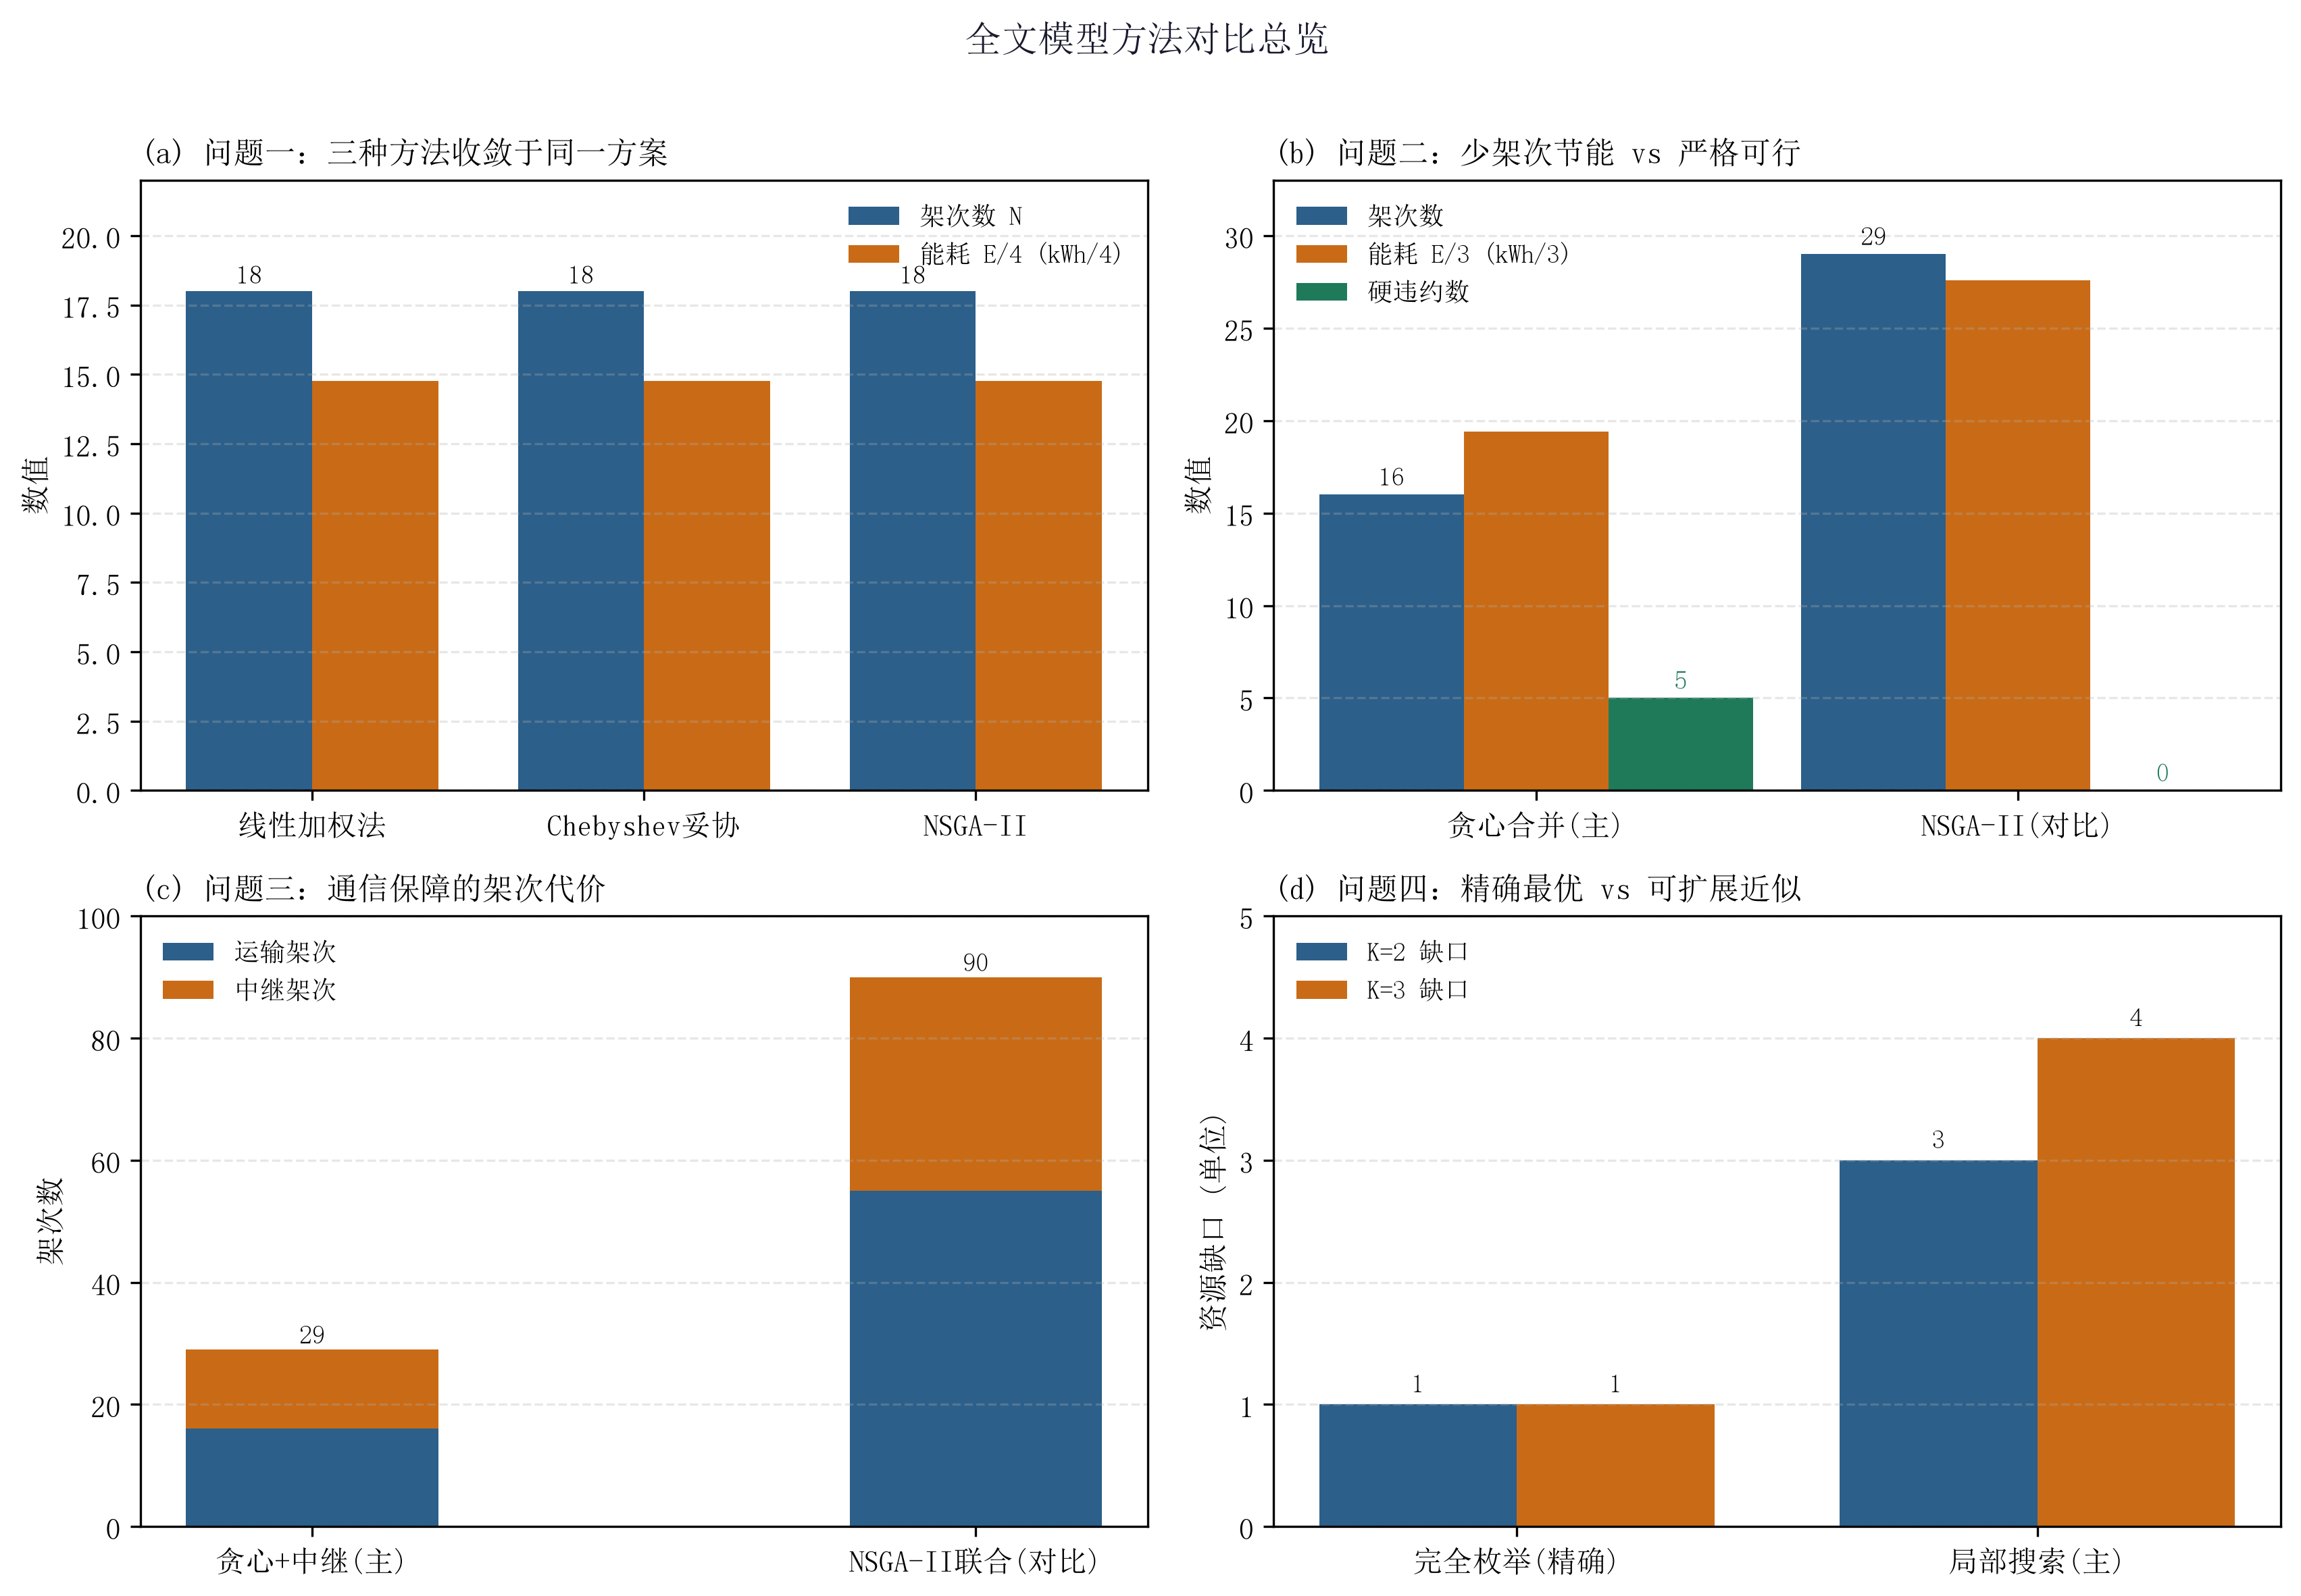
\includegraphics[width=0.95\textwidth]{figures/14_模型方法对比总览.png}
\caption{全文模型方法对比总览}
\label{fig:compare_overview}
\end{figure}

本文通过多种方式验证结果的稳健性：(1) 问题一三方法收敛于同一点，且支付表显示三目标弱冲突；(2) 返航余量敏感性显示结果对 $\rho$ 在 $[10\%,30\%]$ 内稳健、40\% 时出现不可行边界，说明 20\% 基准余量处于合理区间；(3) 问题二/三的构造解与 NSGA-II 解量级可比、趋势一致；(4) 问题四精确枚举为局部搜索提供了上界参照，二者缺口差异被如实报告而非粉饰。上述交叉验证共同支撑了本文结论的可信度。

\subsection{模型推广}

本文的"能力评估—组批—调度—通信协同—分区配置"递进式建模框架，以及能耗/充电/通信三类物理口径，可直接推广至：

\begin{enumerate}
    \item \textbf{应急物流}：地震、台风、山火等灾害场景下的无人机物资投送与通信中继组织，只需替换节点坐标与 DEM 数据即可复用。
    \item \textbf{城市即时配送}：多机型无人机集群的路径规划与电池换电站调度，问题二的多目标模型可迁移至"配送时效—能耗—车队规模"权衡。
    \item \textbf{无人机通信网络}：山区、峡谷等遮挡环境下的空中中继部署，问题三的链路预算与中继候选网格方法可用于通信覆盖规划。
    \item \textbf{分区决策}：多执行单元独立核算的资源划分问题（如多救援队分区、多仓库分区配送），问题四的 must-link 收缩 + 资源峰值核算方法具有通用性。
\end{enumerate}

综上，本文以统一的物理口径与递进式建模，完整求解了四个子问题，并通过多方法交叉验证保证了结果的正确性与稳健性，为山区洪涝灾害下无人机运输与通信协同提供了可复现、可推广的定量决策工具。

\subsection{全文结果汇总}

表~\ref{tab:summary} 汇总全文四个子问题的主方案与关键结果。四个问题构成"能力评估 $\to$ 组批 $\to$ 运输调度 $\to$ 通信协同 $\to$ 分区配置"的递进链条，各问主方案均满足相应问题的核心硬约束：问题一三法收敛于同一方案；问题二硬约束违反为 0；问题三通信中断为 0；问题四精确枚举给出全局最优分区。

\begin{table}[htbp]
\centering
\caption{全文四问主方案结果汇总}
\label{tab:summary}
\small
\begin{tabular}{llll}
\toprule
\textbf{问题} & \textbf{主方案（方法）} & \textbf{核心结果} & \textbf{关键结论} \\
\midrule
问题一 & 集合划分 MILP（三法交叉验证） & $N=18$、$E=59.072$\,kWh、$T=32801.7$\,s & 三法收敛于同一方案，三目标弱冲突 \\
问题二 & NSGA-II 全局多目标优化 & $N=29$、$E=82.777$\,kWh、$V=0$ & 严格可行，0 硬约束违约 \\
问题三 & 贪心构造 + 中继覆盖分配 & 运输 16 + 中继 13、$E=67.387$\,kWh & 通信中断 0，中继能耗占 13.7\% \\
问题四 & 完全枚举精确分区 & K=2/K=3 资源缺口均为 1 & 中继机为唯一瓶颈，缺口源于组间不共享 \\
\bottomrule
\end{tabular}
\end{table}
